\documentclass{article}\usepackage[]{graphicx}\usepackage[]{color}
% maxwidth is the original width if it is less than linewidth
% otherwise use linewidth (to make sure the graphics do not exceed the margin)
\makeatletter
\def\maxwidth{ %
  \ifdim\Gin@nat@width>\linewidth
    \linewidth
  \else
    \Gin@nat@width
  \fi
}
\makeatother

\definecolor{fgcolor}{rgb}{0.345, 0.345, 0.345}
\newcommand{\hlnum}[1]{\textcolor[rgb]{0.686,0.059,0.569}{#1}}%
\newcommand{\hlstr}[1]{\textcolor[rgb]{0.192,0.494,0.8}{#1}}%
\newcommand{\hlcom}[1]{\textcolor[rgb]{0.678,0.584,0.686}{\textit{#1}}}%
\newcommand{\hlopt}[1]{\textcolor[rgb]{0,0,0}{#1}}%
\newcommand{\hlstd}[1]{\textcolor[rgb]{0.345,0.345,0.345}{#1}}%
\newcommand{\hlkwa}[1]{\textcolor[rgb]{0.161,0.373,0.58}{\textbf{#1}}}%
\newcommand{\hlkwb}[1]{\textcolor[rgb]{0.69,0.353,0.396}{#1}}%
\newcommand{\hlkwc}[1]{\textcolor[rgb]{0.333,0.667,0.333}{#1}}%
\newcommand{\hlkwd}[1]{\textcolor[rgb]{0.737,0.353,0.396}{\textbf{#1}}}%
\let\hlipl\hlkwb

\usepackage{framed}
\makeatletter
\newenvironment{kframe}{%
 \def\at@end@of@kframe{}%
 \ifinner\ifhmode%
  \def\at@end@of@kframe{\end{minipage}}%
  \begin{minipage}{\columnwidth}%
 \fi\fi%
 \def\FrameCommand##1{\hskip\@totalleftmargin \hskip-\fboxsep
 \colorbox{shadecolor}{##1}\hskip-\fboxsep
     % There is no \\@totalrightmargin, so:
     \hskip-\linewidth \hskip-\@totalleftmargin \hskip\columnwidth}%
 \MakeFramed {\advance\hsize-\width
   \@totalleftmargin\z@ \linewidth\hsize
   \@setminipage}}%
 {\par\unskip\endMakeFramed%
 \at@end@of@kframe}
\makeatother

\definecolor{shadecolor}{rgb}{.97, .97, .97}
\definecolor{messagecolor}{rgb}{0, 0, 0}
\definecolor{warningcolor}{rgb}{1, 0, 1}
\definecolor{errorcolor}{rgb}{1, 0, 0}
\newenvironment{knitrout}{}{} % an empty environment to be redefined in TeX

\usepackage{alltt}
\IfFileExists{upquote.sty}{\usepackage{upquote}}{}
\begin{document}

\begin{knitrout}
\definecolor{shadecolor}{rgb}{0.969, 0.969, 0.969}\color{fgcolor}\begin{kframe}
\begin{alltt}
\hlkwd{library}\hlstd{(tidyverse)}
\end{alltt}


{\ttfamily\noindent\itshape\color{messagecolor}{\#\# -- Attaching packages --------------------------------------- tidyverse 1.3.0 --}}

{\ttfamily\noindent\itshape\color{messagecolor}{\#\# v ggplot2 3.3.3\ \ \ \  v purrr\ \  0.3.4\\\#\# v tibble\ \ 3.1.0\ \ \ \  v dplyr\ \  1.0.5\\\#\# v tidyr\ \  1.1.3\ \ \ \  v stringr 1.4.0\\\#\# v readr\ \  1.4.0\ \ \ \  v forcats 0.5.1}}

{\ttfamily\noindent\itshape\color{messagecolor}{\#\# -- Conflicts ------------------------------------------ tidyverse\_conflicts() --\\\#\# x dplyr::filter() masks stats::filter()\\\#\# x dplyr::lag()\ \ \ \ masks stats::lag()}}\begin{alltt}
\hlkwd{library}\hlstd{(targets)}
\hlkwd{library}\hlstd{(glue)}
\end{alltt}


{\ttfamily\noindent\itshape\color{messagecolor}{\#\# \\\#\# Attaching package: 'glue'}}

{\ttfamily\noindent\itshape\color{messagecolor}{\#\# The following object is masked from 'package:dplyr':\\\#\# \\\#\#\ \ \ \  collapse}}\end{kframe}
\end{knitrout}


\begin{knitrout}
\definecolor{shadecolor}{rgb}{0.969, 0.969, 0.969}\color{fgcolor}\begin{kframe}
\begin{alltt}
\hlstd{withr}\hlopt{::}\hlkwd{with_dir}\hlstd{(here}\hlopt{::}\hlkwd{here}\hlstd{(), \{}
  \hlkwd{tar_load}\hlstd{(hpp_dat)}
  \hlkwd{tar_load}\hlstd{(models)}

\hlstd{\})}
\end{alltt}
\end{kframe}
\end{knitrout}

Hello, world.

\section{networks}

\begin{knitrout}
\definecolor{shadecolor}{rgb}{0.969, 0.969, 0.969}\color{fgcolor}\begin{kframe}
\begin{alltt}
\hlstd{models} \hlopt
  \hlkwd{map}\hlstd{(}\hlkwc{.f} \hlstd{=} \hlkwa{function}\hlstd{(}\hlkwc{this_model}\hlstd{)\{}
    \hlstd{outcome} \hlkwb{<-} \hlstd{this_model} \hlopt \hlkwd{pluck}\hlstd{(}\hlstr{"outcome"}\hlstd{)}

    \hlstd{this_model} \hlopt
      \hlkwd{pluck}\hlstd{(}\hlstr{"network"}\hlstd{)} \hlopt
      \hlkwd{plot}\hlstd{()} \hlopt{+}
      \hlkwd{labs}\hlstd{(}
        \hlkwc{title} \hlstd{= outcome,}
        \hlkwc{subtitle} \hlstd{=} \hlstr{"direct evidence comparisons"}
      \hlstd{)}
  \hlstd{\})}
\end{alltt}
\begin{verbatim}
## $model_binom_43448096
\end{verbatim}
\end{kframe}
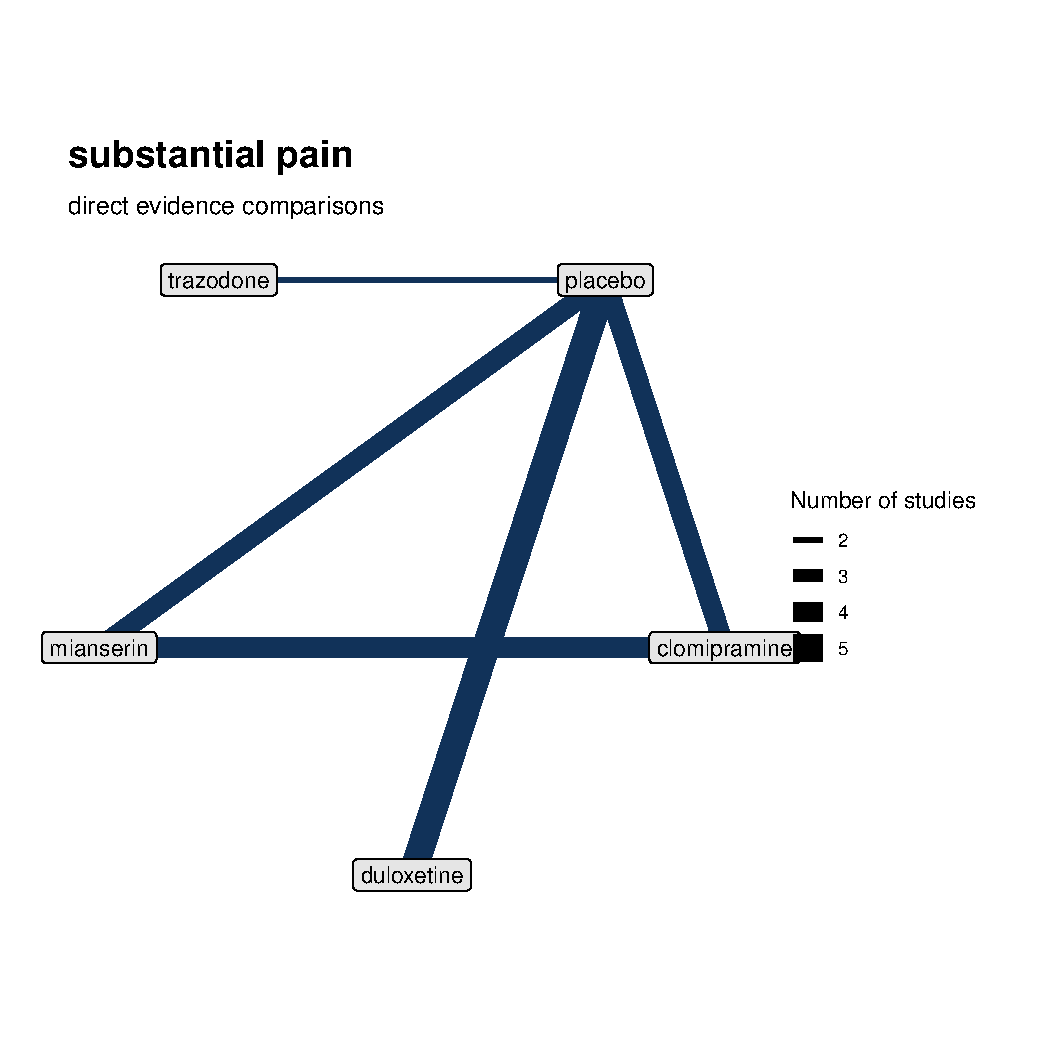
\includegraphics[width=\textwidth]{figure/networks-1} 
\begin{kframe}\begin{verbatim}
## 
## $model_binom_df381d93
\end{verbatim}
\end{kframe}
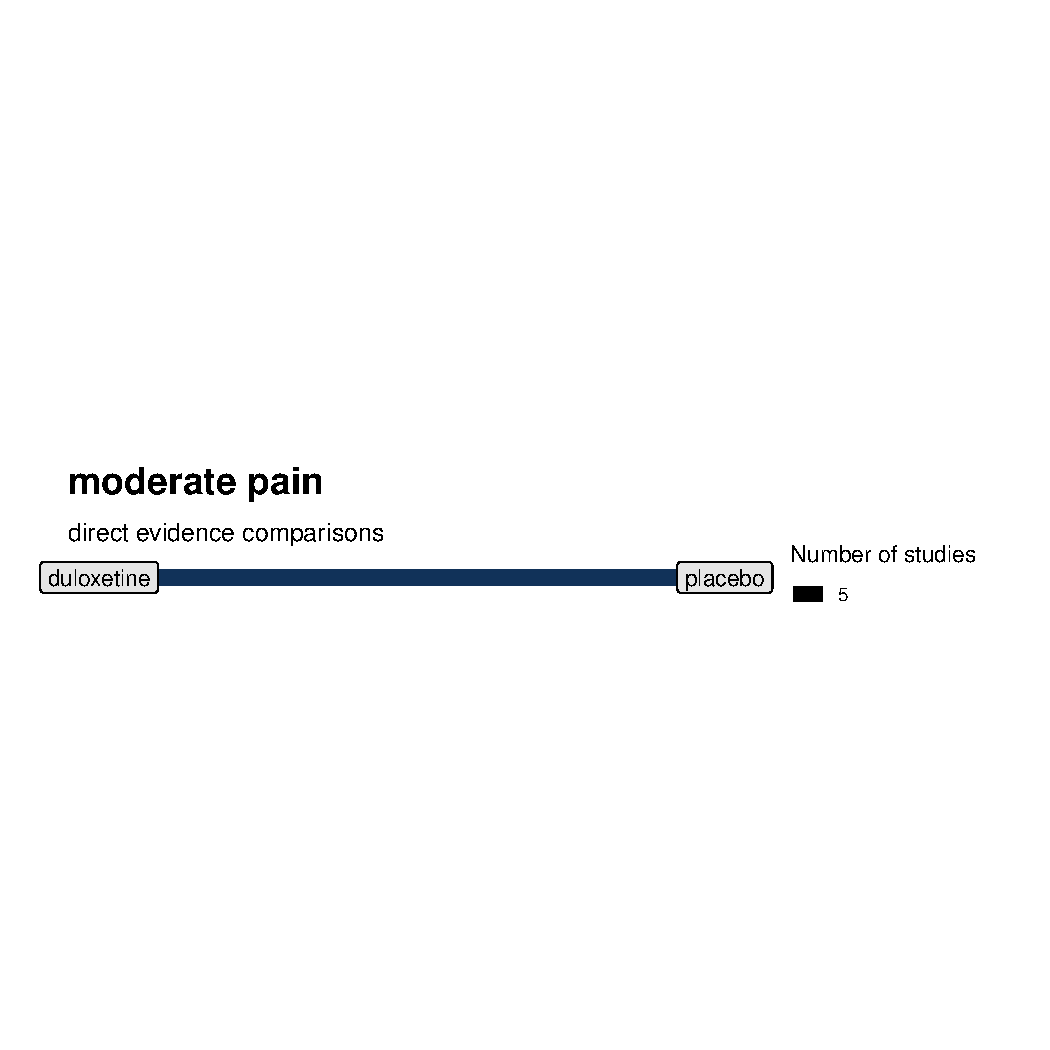
\includegraphics[width=\textwidth]{figure/networks-2} 
\begin{kframe}\begin{verbatim}
## 
## $model_smd_a56a0319
\end{verbatim}
\end{kframe}
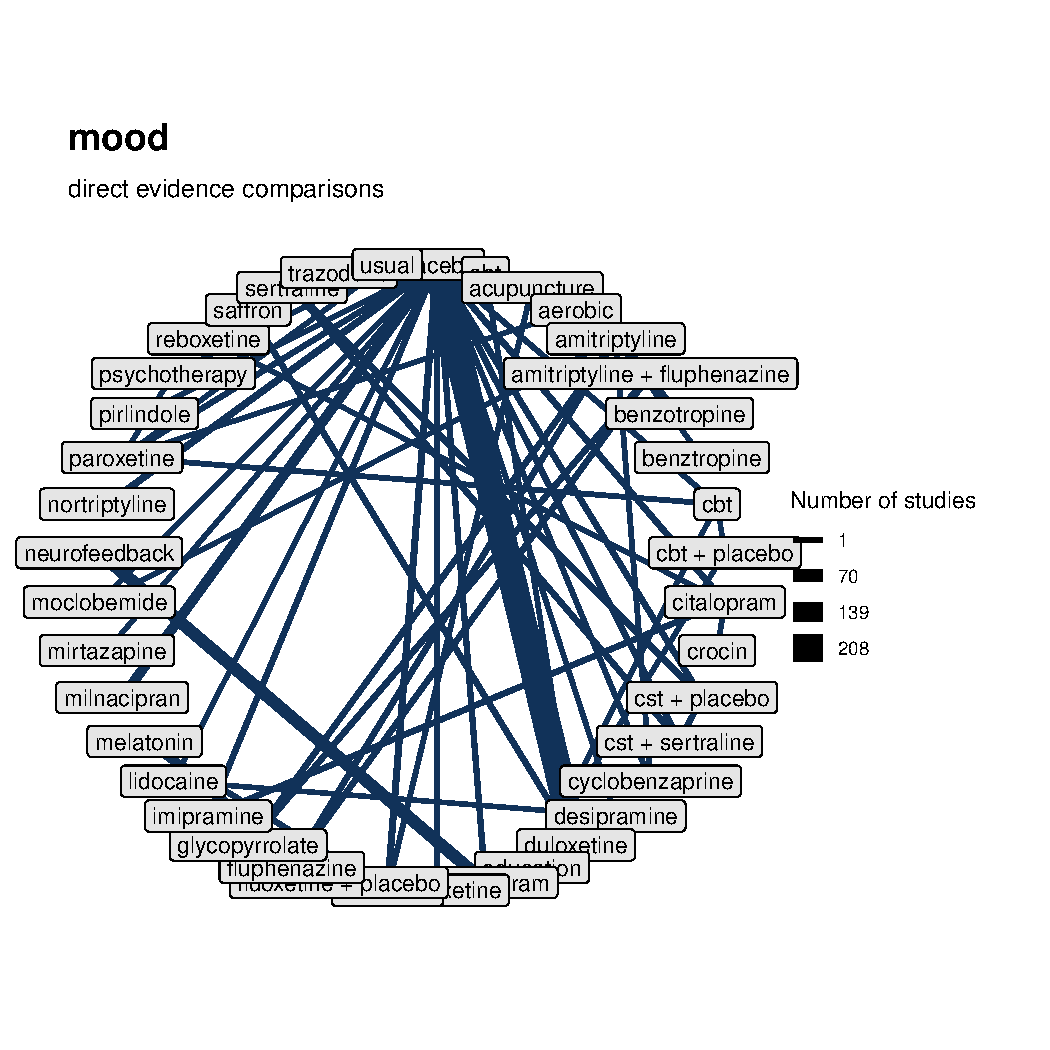
\includegraphics[width=\textwidth]{figure/networks-3} 
\begin{kframe}\begin{verbatim}
## 
## $model_smd_729faf21
\end{verbatim}
\end{kframe}
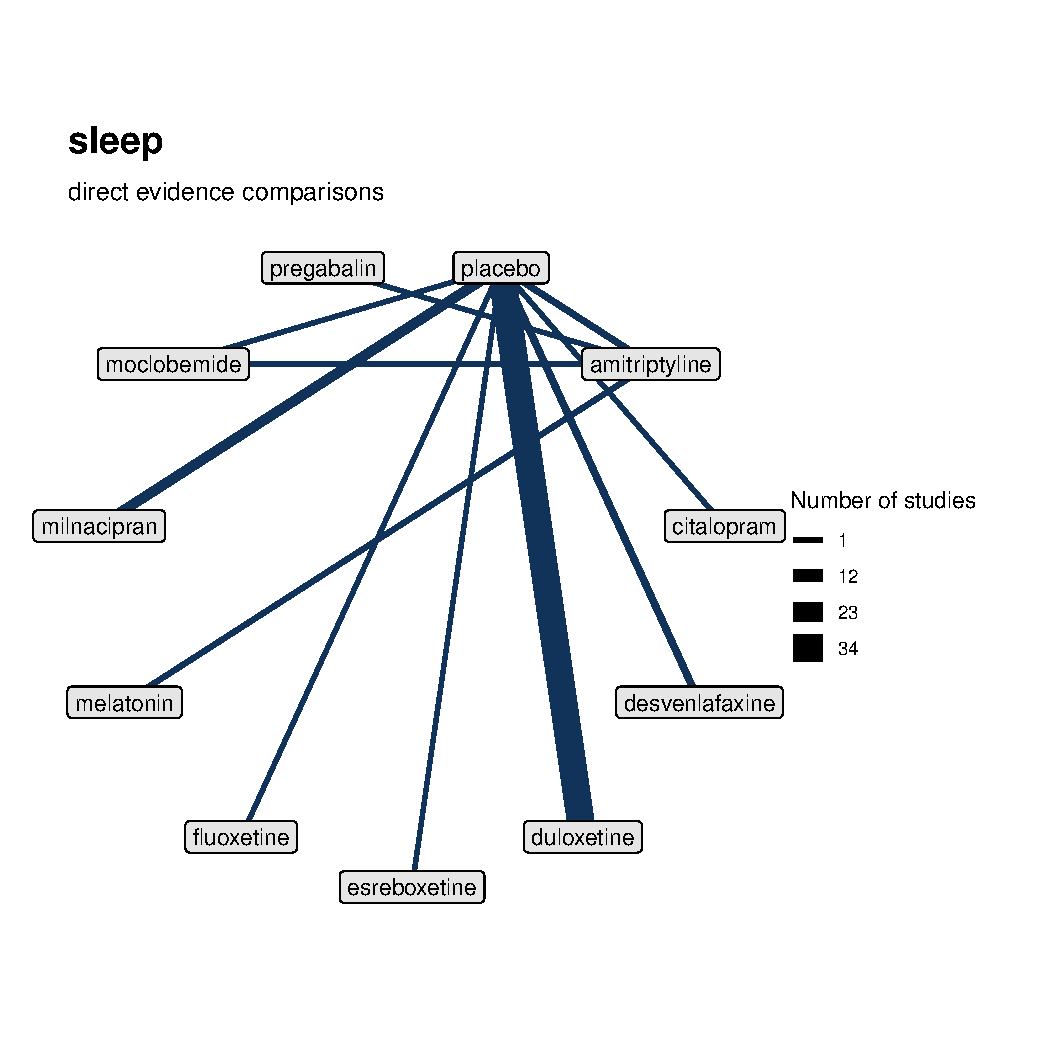
\includegraphics[width=\textwidth]{figure/networks-4} 
\begin{kframe}\begin{verbatim}
## 
## $model_smd_364aa3b7
\end{verbatim}
\end{kframe}
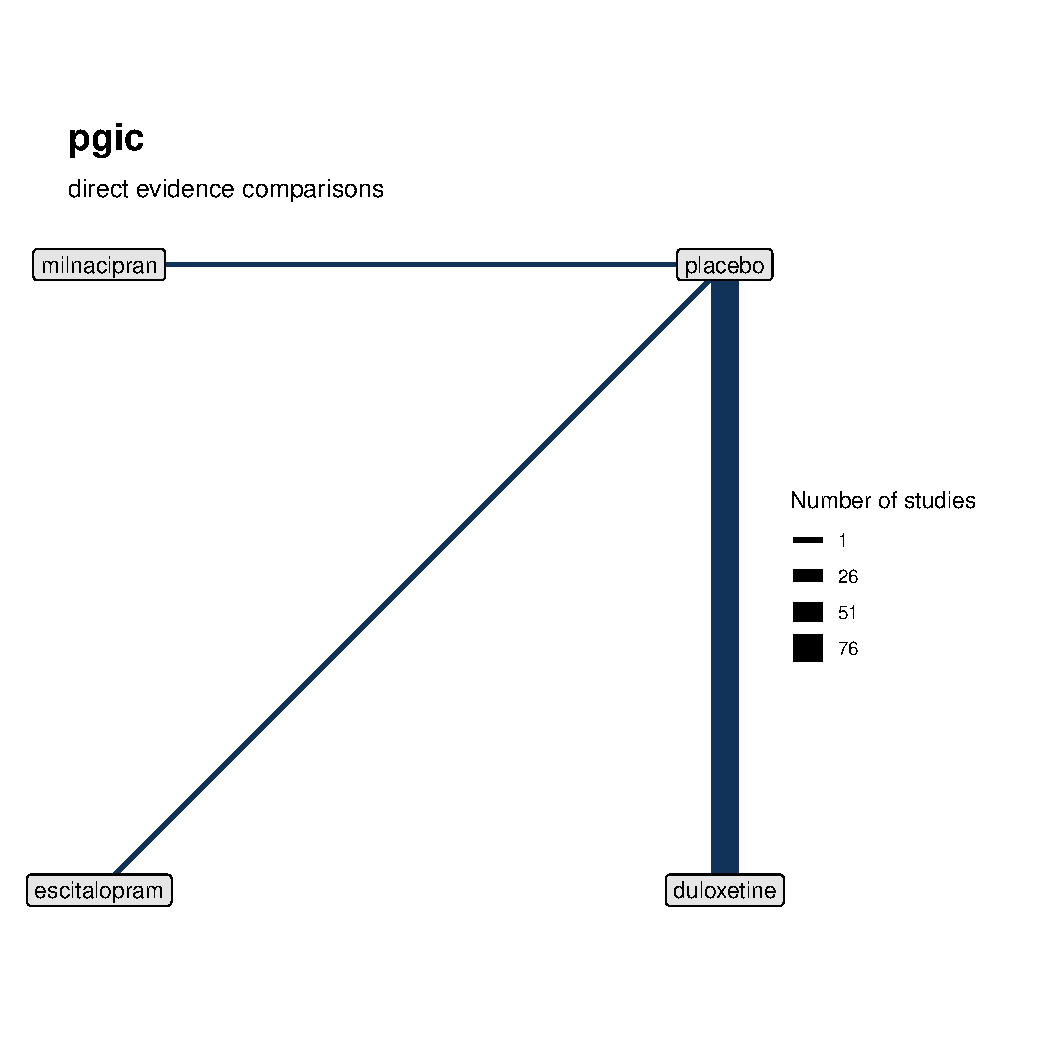
\includegraphics[width=\textwidth]{figure/networks-5} 
\begin{kframe}\begin{verbatim}
## 
## $model_smd_cff505ca
\end{verbatim}
\end{kframe}
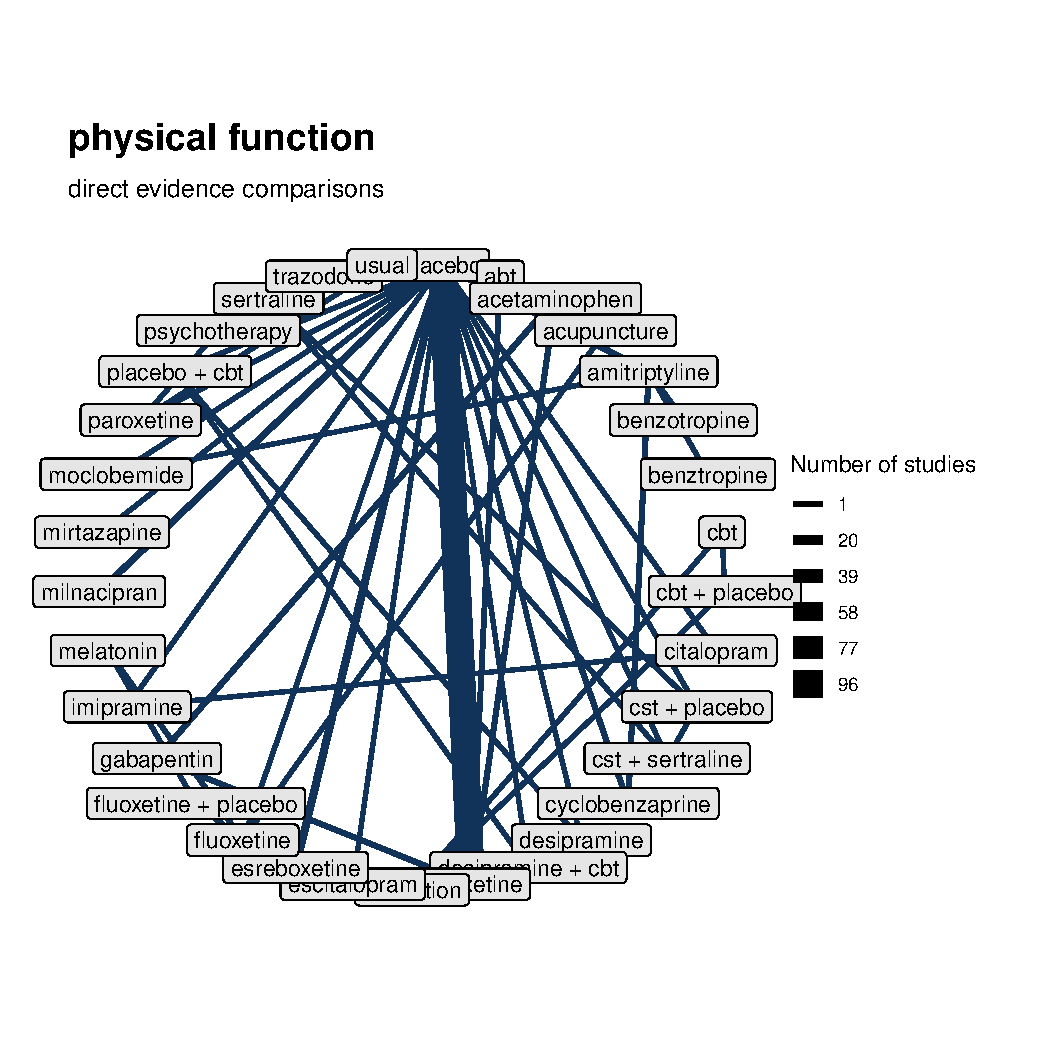
\includegraphics[width=\textwidth]{figure/networks-6} 
\begin{kframe}\begin{verbatim}
## 
## $model_smd_fb9e93c1
\end{verbatim}
\end{kframe}
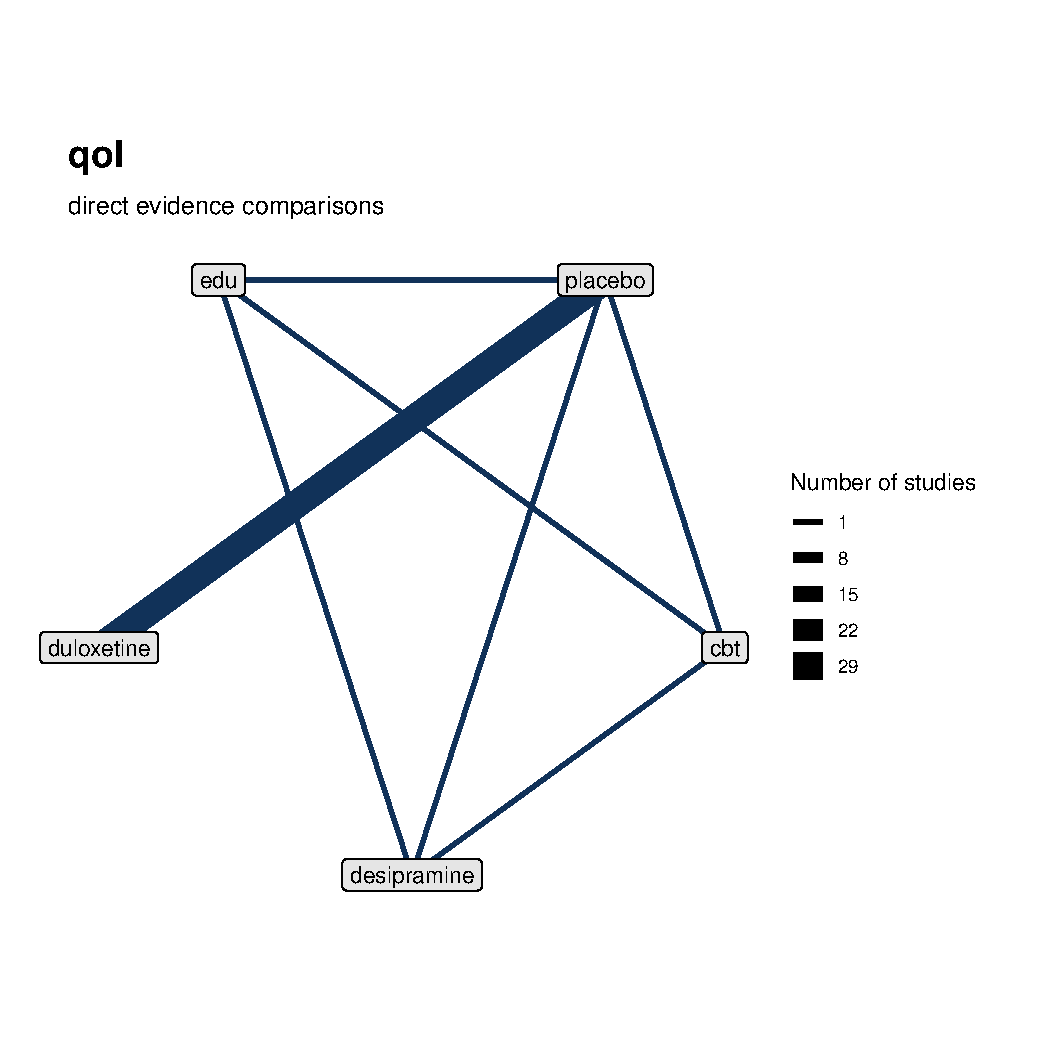
\includegraphics[width=\textwidth]{figure/networks-7} 
\begin{kframe}\begin{verbatim}
## 
## $model_smd_1e5fe681
\end{verbatim}
\end{kframe}
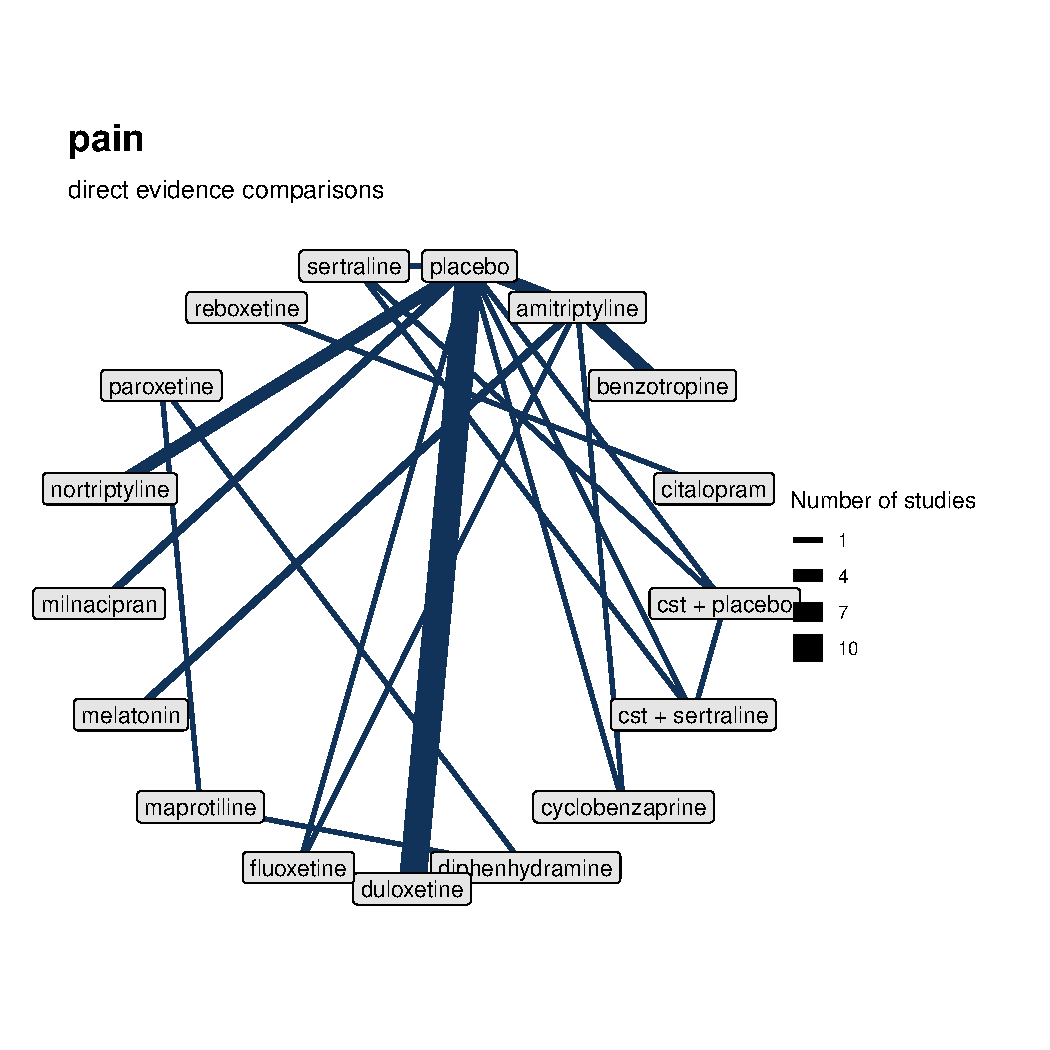
\includegraphics[width=\textwidth]{figure/networks-8} 


\end{knitrout}



\end{document}
